
\documentclass[hyperref={pdfpagelabels=false},ngerman]{beamer}

% stop font warning
\let\Tiny=\tiny
\providecommand\thispdfpagelabel[1]{}

\usepackage[english]{babel}
\usepackage{lmodern}
\usepackage[T1]{fontenc}
\usepackage[utf8]{inputenc}
\usepackage{graphicx,import}
\usepackage{feynmp}
\DeclareGraphicsRule{*}{mps}{*}{} 
\DeclareGraphicsExtensions{.pdf}
\usepackage{amsmath,amssymb,amstext,amsfonts} % mathrsfs
\usepackage{array,booktabs,tabularx}
\usepackage{tikz,tikz-uml,pgf-pie}
\usetikzlibrary{shapes,calc,arrows,positioning}
\tikzstyle{block} = [rectangle, draw, text width=7em, text centered, minimum height=2em]
\tikzstyle{arrow} = [draw, -latex, thick]
\tikzstyle{arrow2} = [draw, latex-latex, thick]
\tikzstyle{quark}  = [rectangle, draw, fill=yellow, minimum width=2em, text centered, minimum height=2em]
\tikzstyle{lepton} = [rectangle, draw, fill=red!50, minimum width=2em, text centered, minimum height=2em]
\tikzstyle{gauge}  = [circle   , draw, fill=green , minimum size=2em, inner sep=0pt, text centered]
\tikzstyle{scalar} = [diamond  , draw, fill=blue!40, minimum width=2.3em, text centered, minimum height=2.3em, inner sep=0pt]
\tikzstyle{goldstone} = [diamond, draw, dashed, fill=blue!30, minimum width=2.3em, text centered, minimum height=2.3em, inner sep=0pt]
\tikzstyle{squark}   = [diamond, draw, fill=yellow, minimum width=2.3em, text centered, minimum height=2.3em, inner sep=0pt]
\tikzstyle{slepton}  = [diamond, draw, fill=red!50, minimum width=2.3em, text centered, minimum height=2.3em, inner sep=0pt]
\tikzstyle{gaugino}  = [rectangle, draw, fill=green , minimum size=2em, inner sep=0pt, text centered]
\tikzstyle{higgsino} = [rectangle, draw, fill=blue!40  , minimum width=2em, text centered, minimum height=2em]
\tikzstyle{inert}    = [diamond  , draw, fill=teal!80, minimum width=2.3em, text centered, minimum height=2.3em, inner sep=0pt]
\tikzstyle{inertino} = [rectangle, draw, fill=teal!80, minimum width=2em, text centered, minimum height=2em]
\tikzstyle{graviton} = [regular polygon, regular polygon sides=5, draw, fill=orange!80, minimum width=2em, text centered, minimum height=2em]
\tikzstyle{gravitino} = [regular polygon, regular polygon sides=8, draw, fill=orange!80, minimum width=2em, text centered, minimum height=2em]
\tikzstyle{phantom}  = [rectangle, minimum width=2em, text centered, minimum height=2em]
\usepackage{slashed}
\usepackage{fixltx2e} % textsubscript
\usepackage{multirow}
\usepackage{tcolorbox}
\usepackage{pifont}
\usepackage{xspace}
\usepackage{hyperref}
\hypersetup{colorlinks,linkcolor=,urlcolor=blue}
\usepackage{listings}
\lstset{breaklines=true,
  breakatwhitespace=true,
%  numbers=left,
  numberstyle=\tiny,
  stepnumber=1,
  basicstyle=\ttfamily\footnotesize,
  commentstyle=\ttfamily\color{gray},
  postbreak={\mbox{{$\hookrightarrow$}}\space\space},
  breakindent=10pt,
  breakautoindent=false,
  showspaces=false,
  showstringspaces=false,
  frame=single}

\definecolor{darkgreen}{RGB}{0,176,0}

\newcommand{\cmark}{\ding{51}}%
\newcommand{\xmark}{\ding{55}}%
\newcommand{\fmfvcenter}[1]{\;\vcenter{\hbox{\fmfreuse{#1}}}\;}
\newcommand{\eh}[1]{\,\mathsf{#1}}
\newcommand{\ok}{\textcolor{darkgreen}{\cmark}}
\newcommand{\notok}{\textcolor{red}{\xmark}}
\newcommand{\maybe}{\textcolor{gray}{\cmark}}
\newcommand{\meh}{\textcolor{gray}{\textbf{\huge\lower.1em\hbox{-}}}}
\newcommand{\Lagr}{\mathcal{L}}
\newcommand{\MS}{\ensuremath{M_S}}
\newcommand{\mathi}{\mathsf{i}}
\newcommand{\mycite}[1]{\ensuremath{\text{\textcolor{darkgray}{\tiny [#1]}}}}
\newcommand{\bigcite}[1]{\textcolor{darkgray}{[#1]}}
\newcommand{\dimrep}[1]{\mathbf{#1}}
\newcommand{\dimrepadj}[1]{\mathbf{\overline{#1}}}
\newcommand{\ESSM}{E\textsubscript{6}SSM}
\newcommand{\CESSM}{CE\textsubscript{6}SSM}
\DeclareMathOperator{\tildeRe}{\widetilde Re}
\DeclareMathOperator{\sign}{sign}
\DeclareMathOperator{\re}{Re}
\DeclareMathOperator{\im}{Im}
\renewcommand{\emph}[1]{\textbf{\textcolor{darkblue}{#1}}}
\newcommand{\dd}{\mathsf{d}}
\newcommand{\myurl}[1]{\href{#1}{#1}}
\newcommand{\Superpot}{\mathcal{W}}
\newcommand{\SuperField}[1]{#1}
\newcommand{\ConjSuperField}[1]{\bar{#1}}
\newcommand{\UY}{\ensuremath{U(1)_{Y}}}
\newcommand{\UN}{\ensuremath{U(1)_{N}}}
\newcommand{\Uem}{\ensuremath{U(1)_\text{em}}}
\newcommand{\SUL}{\ensuremath{SU(2)_\text{L}}}
\newcommand{\SUc}{\ensuremath{SU(3)_\text{c}}}
\newcommand{\SOten}{\ensuremath{{SO(10)}}}
\newcommand{\comma}{,}
\newcommand{\DRbar}{\ensuremath{\overline{\text{DR}}}}
\newcommand{\DRbarp}{\ensuremath{\overline{\text{DR}}'}}
\newcommand{\MSbar}{\ensuremath{\overline{\text{MS}}}}
\newcommand{\SM}{\ensuremath{\text{SM}}}
\newcommand{\MSSM}{\ensuremath{\text{MSSM}}}
\newcommand{\BSM}{\ensuremath{\text{BSM}}}
\newcommand{\EFT}{\ensuremath{\text{EFT}}\xspace}
\newcommand{\THDM}{\ensuremath{\text{2HDM}}\xspace}
\newcommand{\pole}{\ensuremath{\text{pole}}}
\newcommand{\tree}{\ensuremath{\text{tree}}}
\newcommand{\fsstar}{\textbf{*}}
\newcommand{\FS}{\texttt{FlexibleSUSY}\xspace}
\newcommand{\fsh}{\texttt{FS+H}\xspace}
\newcommand{\feft}{\texttt{FlexibleEFTHiggs}\xspace}
\newcommand{\hssusy}{\texttt{HSSUSY}\xspace}
\newcommand{\Himalaya}{\texttt{Himalaya}\xspace}
\newcommand{\FH}{\texttt{FeynHiggs}\xspace}
\newcommand{\SPheno}{\texttt{SPheno}\xspace}
\newcommand{\SARAH}{\texttt{SARAH}\xspace}
\newcommand{\SOFTSUSY}{\texttt{SOFTSUSY}\xspace}
\newcommand{\Zv}{\ensuremath{\backslash\mkern-11.0mu{Z_3}}}
\newcommand{\downrightknickarrow}{\mathrel{\scalebox{1.3}{\rotatebox[origin=c]{180}{$\Lsh$}}}}
\newcommand{\threelinebrace}{$\left. \begin{array}{c} \\ \\ \\ \end{array} \right\rbrace$}
\newcommand{\fivelinebrace}{$\left. \begin{array}{c} \\ \\ \\ \\ \\ \end{array} \right\rbrace$}
\newcommand{\twolinebrace}{$\left. \begin{array}{c} \\ \\ \end{array} \right\rbrace$}
\newcommand{\elevenlinebrace}{$\left. \begin{array}{c} \\ \\ \\ \\ \\ \\ \\ \\ \\ \\ \\ \end{array} \right\rbrace$}
\newcommand{\at}{\alpha_t}
\newcommand{\ab}{\alpha_b}
\newcommand{\atau}{\alpha_\tau}
\newcommand{\as}{\alpha_s}
\newcommand{\aem}{\alpha_\text{em}}
\newcommand{\GeV}{\eh{GeV}}
\newcommand{\TeV}{\eh{TeV}}
\newcommand{\SQCD}{\ensuremath{\scalefont{.8}\text{SQCD}}}
\newcommand{\Qpole}{\ensuremath{Q_\text{pole}}}
\newcommand{\Qmatch}{\ensuremath{Q_\text{match}}}
\newcommand{\Qsplit}{\ensuremath{Q_\text{split}}\xspace}
\newcommand{\QTHDM}{\ensuremath{Q_\text{\THDM}}\xspace}
\newcommand{\DMh}{\ensuremath{\Delta M_h^{(\text{FO})}}}
\newcommand{\DMhQpole}{\ensuremath{\Delta M_h^{(\Qpole)}}}
\newcommand{\DMhQmatch}{\ensuremath{\Delta M_h^{(\Qmatch)}}}
\newcommand{\DMhMt}{\ensuremath{\Delta M_h^{(m_t)}}}
\newcommand{\DMhAlphaS}{\ensuremath{\Delta M_h^{(\as)}}}
\newcommand{\DMhAlphaEm}{\ensuremath{\Delta M_h^{(\aem)}}}
\newcommand{\DMhHSSUSY}{\ensuremath{\Delta M_h^{(\text{EFT})}}}
\newcommand{\DMhHSSUSYytSM}{\ensuremath{\Delta M_h^{(y_t^\SM)}}}
\newcommand{\DMhHSSUSYytMSSM}{\ensuremath{\Delta M_h^{(y_t^\MSSM)}}}
\newcommand{\DMhEFT}{\ensuremath{\Delta M_h^{(v^2/\MS^2)}}}
\def\HSSUSY{\texttt{HSSUSY}}

% set look of slides
\usetheme{Madrid}
\useoutertheme{default}
\useinnertheme{circles}
\usecolortheme{default}
\beamertemplatenavigationsymbolsempty % keine Navigationselemente
\setbeamersize{text margin left = 1cm, text margin right = 1cm}

% define footer
\makeatletter
\setbeamertemplate{footline}
{
  \hfill\hbox{\insertframenumber{} / \inserttotalframenumber\hspace*{4pt}}%
  \vskip3pt%
}
\makeatother
\usecolortheme{tud}

\title{Precise Higgs mass calculations in BSM models in light of the
  recent LHC results}

\author[Alexander Voigt]{Alexander Voigt}

\date{IKTP-Institutsseminar, TU-Dresden\\[1em]
  13/12/2018}

% \institute[Aachen]{RWTH Aachen}
\subject{FlexibleSUSY,MSSM,Higgs,FlexibleEFTHiggs}
\keywords{FlexibleSUSY,MSSM,Higgs,FlexibleEFTHiggs}

%%%%%%%%%%%%%%%%%%%%%%%%%%%%%%%%%%%%%%%%%%%%%%%%%%%%%%%%%%%%%%%%%%%%%%%%%%%%%

\begin{document}

%%%%%%%%%%%%%%%%%%%%%%%%%%%%%%%%%%%%%%%%%%%%%%%%%%%%%%%%%%%%%%%%%%%%%%%%%%%%%

% Savebox which contains the the Feynman rules
\newsavebox{\feynmanrules}
\sbox{\feynmanrules}{
\begin{fmffile}{Feynman/higgs} % file name and path
  \fmfset{thin}{.8pt}
  \fmfset{wiggly_len}{5mm}
  \fmfset{dash_len}{2.5mm}
  \fmfset{dot_size}{1thick}
  \fmfset{arrow_len}{2.5mm}
  \fmfset{curly_len}{2.5mm}

\begin{fmfgraph*}(60,60)
  \fmfkeep{hX}
  \fmfleft{v1}
  \fmfright{v2}
  \fmf{higgs}{v1,c1}
  \fmf{higgs}{c2,v2}
  \fmf{quark,left,tension=0.5,label=$X$}{c1,c2}
  \fmf{quark,left,tension=0.5}{c2,c1}
\end{fmfgraph*}

\begin{fmfgraph*}(60,60)
  \fmfkeep{htop}
  \fmfleft{v1}
  \fmfright{v2}
  \fmf{higgs}{v1,c1}
  \fmf{higgs}{c2,v2}
  \fmf{quark,left,tension=0.5,label=$t$}{c1,c2}
  \fmf{quark,left,tension=0.5}{c2,c1}
\end{fmfgraph*}

\begin{fmfgraph*}(60,60)
  \fmfkeep{hstop}
  \fmfleft{v1}
  \fmfright{v2}
  \fmf{higgs}{v1,c1}
  \fmf{higgs}{c2,v2}
  \fmf{scalar,left,tension=0.5,label=$\tilde{t}_i$}{c1,c2}
  \fmf{scalar,left,tension=0.5}{c2,c1}
\end{fmfgraph*}

\begin{fmfgraph*}(60,60)
  \fmfkeep{hstopA}
  \fmfleft{v1}
  \fmfright{v2}
  \fmf{higgs}{v1,c,v2}
  \fmf{scalar,right,tension=0.8,label=$\tilde{t}_i$}{c,c}
\end{fmfgraph*}

\begin{fmfgraph*}(60,60)
  \fmfkeep{htoptad}
  \fmfleft{v1}
  \fmfright{v2}
  \fmftop{t1}
  \fmf{higgs}{v1,c,v2}
  \fmffreeze
  \fmf{higgs}{c,c1}
  \fmf{quark,right,tension=0.3,label=$t$}{c1,c2}
  \fmf{quark,right,tension=0.3}{c2,c1}
  \fmf{phantom,tension=10}{c2,t1}
\end{fmfgraph*}

\begin{fmfgraph*}(60,60)
  \fmfkeep{hstoptad}
  \fmfleft{v1}
  \fmfright{v2}
  \fmftop{t1}
  \fmf{higgs}{v1,c,v2}
  \fmffreeze
  \fmf{higgs}{c,c1}
  \fmf{scalar,right,tension=0.3,label=$\tilde{t}_i$}{c1,c2}
  \fmf{scalar,right,tension=0.3}{c2,c1}
  \fmf{phantom,tension=10}{c2,t1}
\end{fmfgraph*}
\end{fmffile}
}

%%%%%%%%%%%%%%%%%%%%%%%%%%%%%%%%%%%%%%%%
\begin{frame}[plain]
  \tikz [remember picture,overlay]
  \node at
    ([yshift=1.3cm,xshift=4cm]current page.south)
    {\includegraphics[height=2cm]{images/RWTH_Logo}};
  \titlepage  
\end{frame}

%%%%%%%%%%%%%%%%%%%%%%%%%%%%%%%%%%%%%%%%
\begin{frame}{Contents}
  \tableofcontents
\end{frame}

%%%%%%%%%%%%%%%%%%%%%%%%%%%%%%%%%%%%%%%%

\section{Introduction}
\subsection{Open questions before/after the Higgs discovery}

\begin{frame}[t]{Open questions before/after the Higgs discovery}
  \begin{columns}
    \column{.3\linewidth}
    \scalebox{0.5}{
    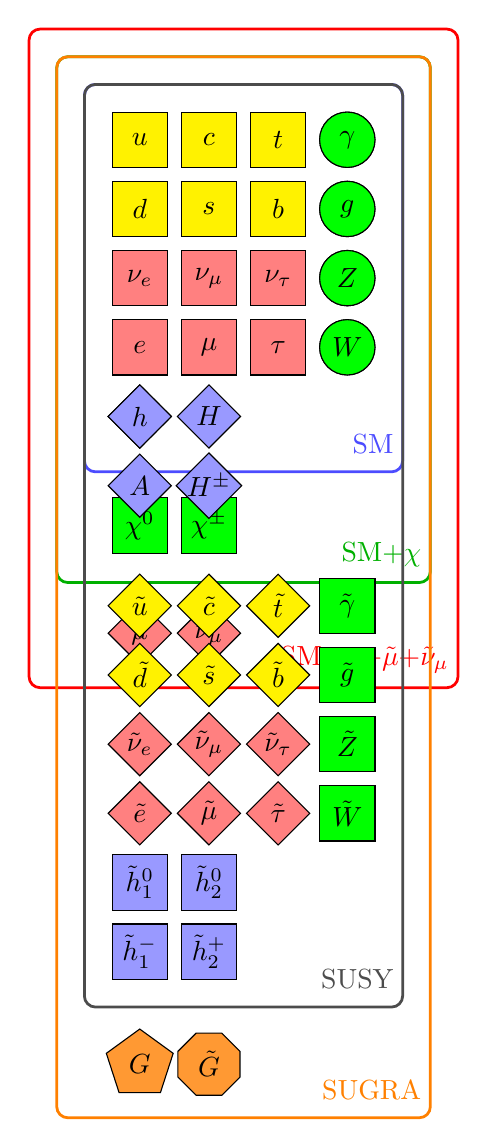
\begin{tikzpicture}[node distance = 2.5em, auto]
      \visible<1-4>{
      \node[quark] (u) {$u$};
      \node[quark, below of=u] (d) {$d$};
      \node[quark, right of=u] (c) {$c$};
      \node[quark, below of=c] (s) {$s$};
      \node[quark, right of=c] (t) {$t$};
      \node[quark, below of=t] (b) {$b$};
      \node[lepton, below of=d] (ne) {$\nu_e$};
      \node[lepton, below of=ne] (e) {$e$};
      \node[lepton, right of=ne] (nm) {$\nu_\mu$};
      \node[lepton, below of=nm] (m) {$\mu$};
      \node[lepton, right of=nm] (nt) {$\nu_\tau$};
      \node[lepton, below of=nt] (ta) {$\tau$};
      \node[gauge, right of=t] (gamma) {$\gamma$};
      \node[gauge, below of=gamma] (g) {$g$};
      \node[gauge, below of=g] (Z) {$Z$};
      \node[gauge, below of=Z] (W) {$W$};
      \node[phantom, below of=W] (corner) {\phantom{X}};
      \node[phantom, below of=corner] (corner2) {\phantom{X}};
      \draw[line width=1, color=blue!70,rounded corners] ($(u) + (-2em,2em)$) rectangle ($(corner) + (2em,-2em)$);
      \node[color=blue!70, anchor=east] (MSSM) at ($(corner.east) + (1em,-1em)$) {SM};
      }
      \visible<1>{
        \node[scalar, fill=blue!10, dashed, below of=e] (h) {$h$};
      }
      \visible<2-4>{
        \node[scalar, below of=e] (h) {$h$};
      }
      \visible<3-4>{
        \node[gaugino, below=1.75em of h] (chi0) {$\chi^{0}$};
        \node[gaugino, right of=chi0] (chipm) {$\chi^{\pm}$};
        \draw[line width=1, color=darkgreen,rounded corners] ($(u) + (-3em,3em)$) rectangle ($(corner2) + (3em,-3.5em)$);
        \node[color=darkgreen, anchor=east] (Split) at ($(corner2.east) + (2em,-2.5em)$) {SM+$\chi$};
      }
      \visible<4>{
        \node[slepton, below=1.7em of chi0] (smu) {$\tilde\mu$};
        \node[slepton, right of=smu] (snu) {$\tilde{\nu}_{\mu}$};
        \draw[line width=1, color=red,rounded corners] ($(u) + (-4em,4em)$) rectangle ($(corner2) + (4em,-7.3em)$);
        \node[color=red, anchor=east] (Split) at ($(corner2.east) + (3em,-6.3em)$) {SM+$\chi$+$\tilde{\mu}$+$\tilde{\nu}_\mu$};
      }
      \visible<5->{
        \node[quark] (u) {$u$};
        \node[quark, below of=u] (d) {$d$};
        \node[quark, right of=u] (c) {$c$};
        \node[quark, below of=c] (s) {$s$};
        \node[quark, right of=c] (t) {$t$};
        \node[quark, below of=t] (b) {$b$};
        \node[lepton, below of=d] (ne) {$\nu_e$};
        \node[lepton, below of=ne] (e) {$e$};
        \node[lepton, right of=ne] (nm) {$\nu_\mu$};
        \node[lepton, below of=nm] (m) {$\mu$};
        \node[lepton, right of=nm] (nt) {$\nu_\tau$};
        \node[lepton, below of=nt] (ta) {$\tau$};
        \node[gauge, right of=t] (gamma) {$\gamma$};
        \node[gauge, below of=gamma] (g) {$g$};
        \node[gauge, below of=g] (Z) {$Z$};
        \node[gauge, below of=Z] (W) {$W$};
        \node[scalar, below of=e] (h) {$h$};
        \node[scalar, right of=h] (H) {$H$};
        \node[scalar, below of=h] (A) {$A$};
        \node[scalar, right of=A] (Hpm) {$H^\pm$};
        %
        \node[squark, below=2em of A] (su) {$\tilde u$};
        \node[squark, below of=su] (sd) {$\tilde d$};
        \node[squark, right of=su] (sc) {$\tilde c$};
        \node[squark, below of=sc] (ss) {$\tilde s$};
        \node[squark, right of=sc] (st) {$\tilde t$};
        \node[squark, below of=st] (sb) {$\tilde b$};
        \node[slepton, below of=sd] (sne) {$\tilde \nu_e$};
        \node[slepton, below of=sne] (se) {$\tilde e$};
        \node[slepton, right of=sne] (snm) {$\tilde \nu_\mu$};
        \node[slepton, below of=snm] (sm) {$\tilde \mu$};
        \node[slepton, right of=snm] (snt) {$\tilde \nu_\tau$};
        \node[slepton, below of=snt] (sta) {$\tilde \tau$};
        \node[gaugino, right of=st] (sgamma) {$\tilde \gamma$};
        \node[gaugino, below of=sgamma] (sg) {$\tilde g$};
        \node[gaugino, below of=sg] (sZ) {$\tilde Z$};
        \node[gaugino, below of=sZ] (sW) {$\tilde W$};
        \node[higgsino, below of=se] (sh) {$\tilde h_1^0$};
        \node[higgsino, right of=sh] (sH) {$\tilde h_2^0$};
        \node[higgsino, below of=sh] (sA) {$\tilde h^-_1$};
        \node[higgsino, below of=sH] (sHpm) {$\tilde h^+_2$};
        \node[phantom, below of=sW    ] (sZprime) {\phantom{X}};
        \node[phantom, below of=sZprime] (corner) {\phantom{X}};
        \node[phantom, below of=corner] (corner2) {\phantom{X}};
        %
        \draw[line width=1, color=black!70,rounded corners] ($(u) + (-2em,2em)$) rectangle ($(corner) + (2em,-2em)$);
        \node[color=black!70, anchor=east] (SUSY) at ($(corner.east) + (1em,-1em)$) {SUSY};
      }
      \visible<6->{
        \node[graviton, below=1.75em of sA] (G) {$G$};
        \node[gravitino, right of=G] (sG) {$\tilde{G}$};
        \draw[line width=1, color=orange, rounded corners] ($(u) + (-3em,3em)$) rectangle ($(corner2) + (3em,-3.5em)$);
        \node[color=orange, anchor=east] (SUGRA) at ($(corner2.east) + (2em,-2.5em)$) {SUGRA};
      }
    \end{tikzpicture}}
    \column{.7\linewidth}
    \emph{Open questions:}\\
    \begin{itemize}
    \item {\color<2->{darkgreen}{Does the Higgs exist?}}
    \item {\color<3->{darkgreen}{What does DM consist of?}}
    \item {\color<4->{darkgreen}{What causes the deviation of $(g-2)_\mu$?}}
    \item {\color<5->{darkgreen}{Is the vacuum stable up to $M_{\text{Pl}}$?}}
    \item {\color<5->{darkgreen}{Why is $M_h = 125\eh{GeV}$?}}
    \item {\color<5->{darkgreen}{Is there a solution to the hierarchy problem?}}
    \item {\color<6->{darkgreen}{Can QFT and gravity be unified?}}
    \end{itemize}
  \end{columns}
\end{frame}

\subsection{Advantages/disadvantages of SUSY}

\begin{frame}{Problem 1: no SUSY particles observed}
  \begin{center}
    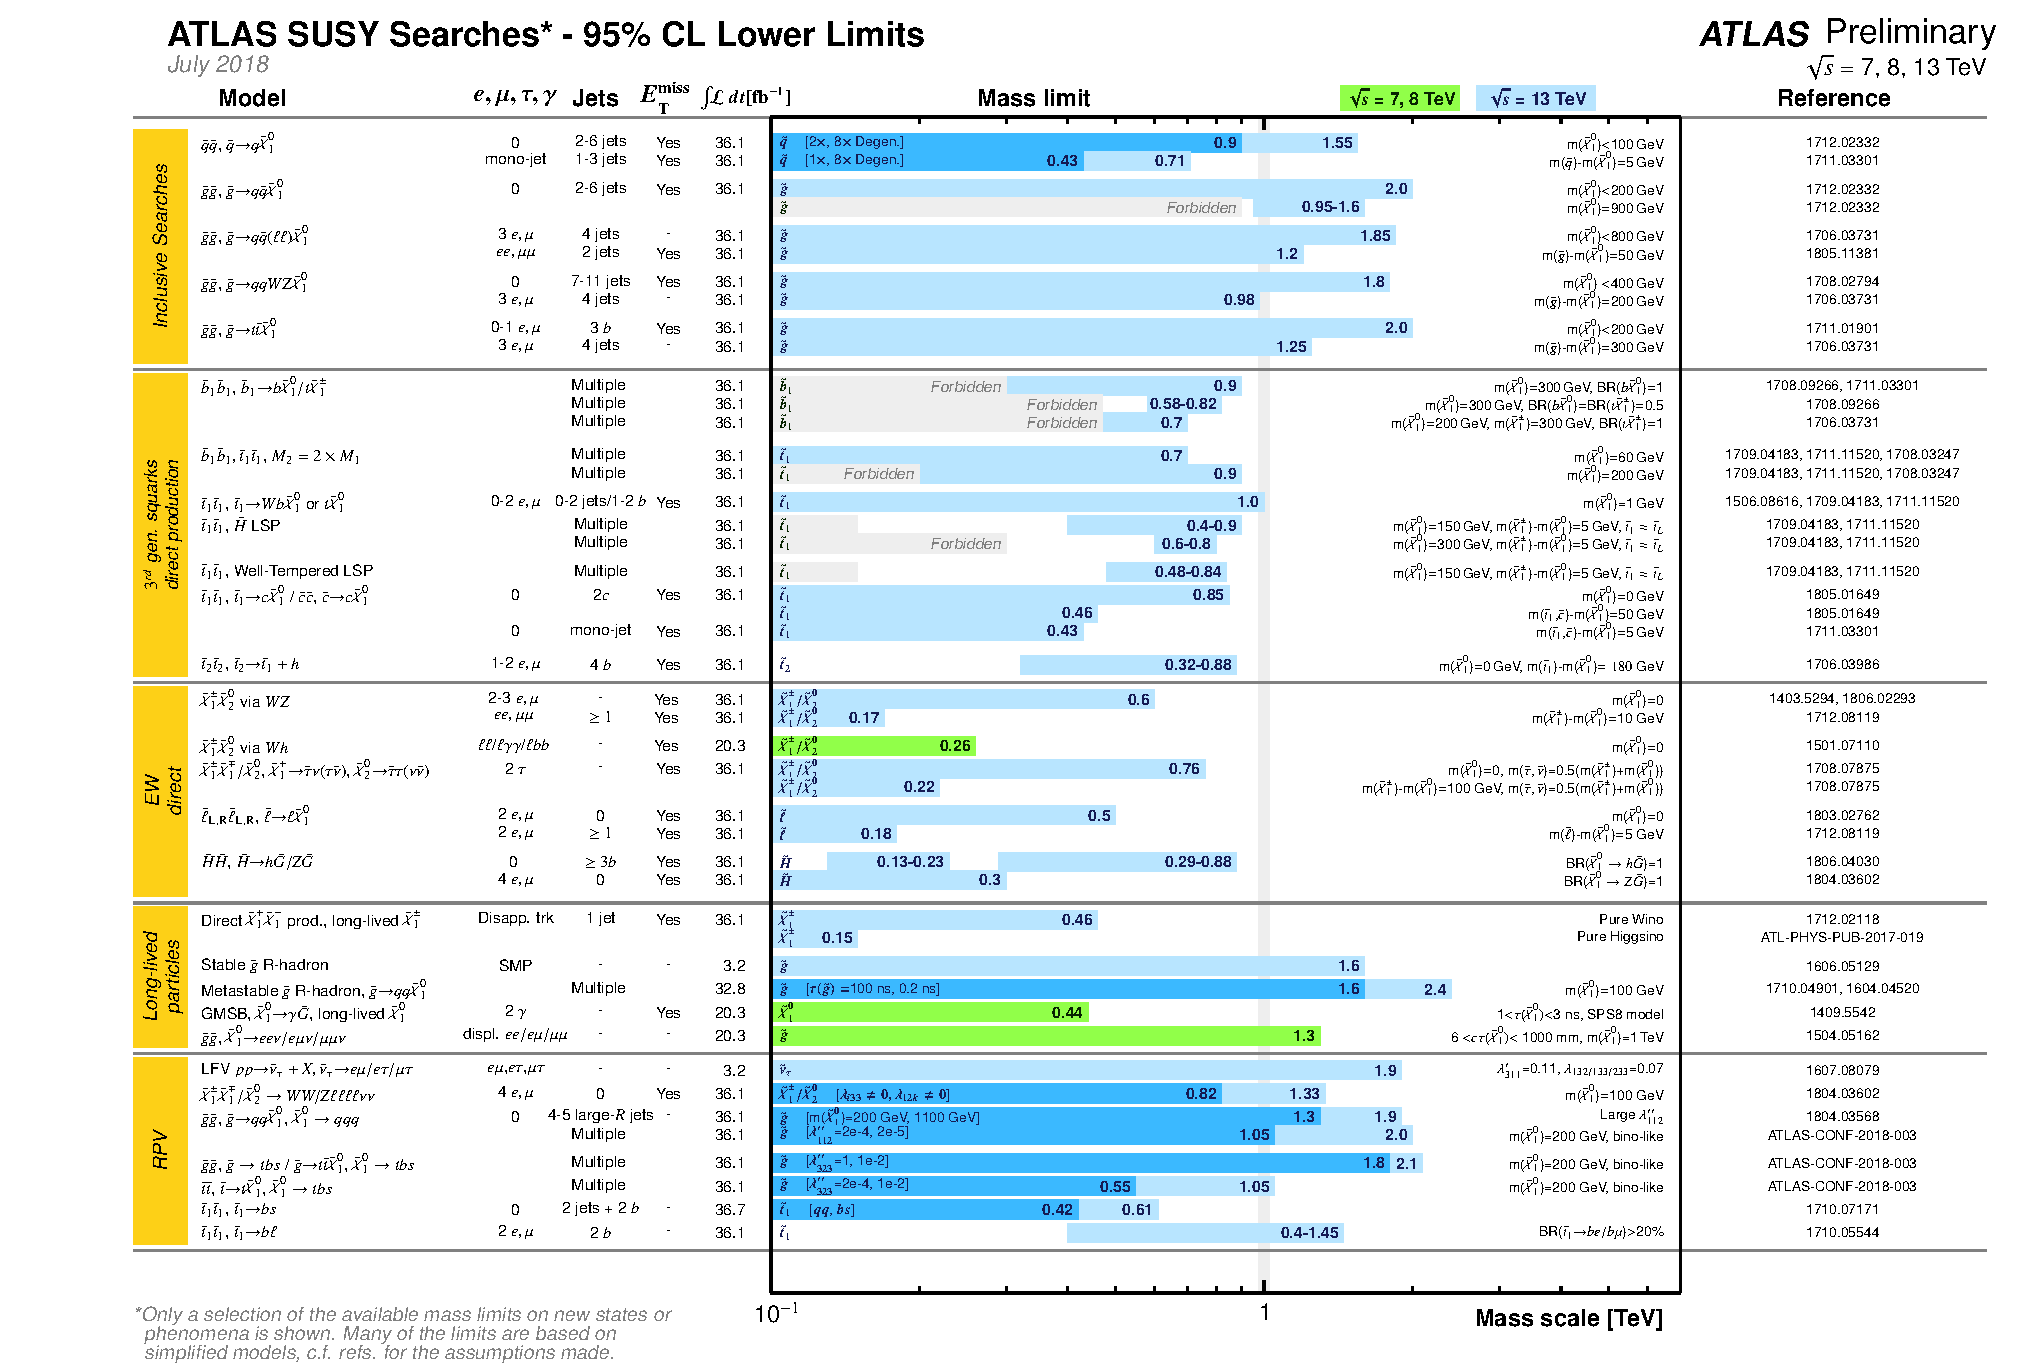
\includegraphics[width=\textwidth]{images/ATLAS_SUSY_Summary}
  \end{center}
\end{frame}

\begin{frame}{Problem 2: Tree-level Higgs mass too small}
  (minimal) SUSY \emph{predicts} at tree-level:
  \begin{align*}
    m_h = m_Z |\cos 2\beta| \le m_Z
  \end{align*}
  But from experiment we know:
  \begin{align*}
    M_h &\approx 125.09 \GeV \\
    M_Z &\approx 91.2 \GeV
  \end{align*}
  $\Rightarrow$ \emph{large loop corrections} required!
  \begin{align*}
    M_h^2 &= m_h^2 + \Delta m_h^2
    & &\Rightarrow &
    \Delta m_h^2 &\geq (85\eh{GeV})^2
  \end{align*}
\end{frame}

\subsection{How can we test a SUSY model?}

\begin{frame}{How can we test a SUSY model?}
  \emph{Idea:}
  \begin{enumerate}
  \item Calculate $M_h$ as precisely as possible in the SUSY model:
  \begin{align*}
    M_h^2 &= m_h^2 + \Delta m_h^2
  \end{align*}
  \item Constrain the parameter space by requiring:
    \begin{align*}
      M_h \overset{!}{=} 125.09 \GeV \pm \Delta M_h^{\text{exp}} \pm \Delta M_h^{\text{theo}}
    \end{align*}
  \end{enumerate}
  \emph{Problem:} because of large loop corrections $\Delta m_h^2$:
  \begin{align*}
    \Delta M_h^{\text{theo}} &\gtrsim (1\ldots 2)\eh{GeV} \quad \text{at least!} \\
    \Delta M_h^{\text{exp}} &= 0.24\eh{GeV} \ \ \mycite{PDG-2017}
  \end{align*}
\end{frame}

\section{Higgs mass prediction}

\begin{frame}{Contents}
  \tableofcontents[currentsection]
\end{frame}

\begin{frame}{Approaches to predict $M_h$}
  \begin{center}
    \begin{tikzpicture}[scale=0.9]
      \draw[->, thick] (0,0) -- (0,1) node[left]{$M_t$} -- (0,5) node[left]{$\MS$} -- (0,6);
      \node at (2.5,7) {\emph{Fixed order}};
      \draw[thick] (1,0)   rectangle node{SM}    (4,0.9);
      \draw[thick] (1,1.1) rectangle node{MSSM}  (4,6);
      \draw[<-, thick, red] (4.1,5) -- (4.5,5) node[right]{$M_h$};
      \node at (7.5,7) {\emph{Effective Field Theory}};
      \draw[thick] (6,0)   rectangle node{SM}    (9,0.9);
      \draw[thick] (6,1.1) rectangle node{EFT}   (9,4.9);
      \draw[thick] (6,5.1) rectangle node{MSSM}  (9,6);
      \draw[<-, thick, red] (9.1,1.5) -- (9.5,1.5) node[right]{$M_h$};
    \end{tikzpicture}
  \end{center}
\end{frame}

% Argumentation:

% 1. classic approach: FO calculation -> large uncertainty due to
% heavy particles. -> discuss recent status (3-loop) and uncertainty

\subsection{Fixed-order calculation}

\begin{frame}{Contents}
  \tableofcontents[currentsection,currentsubsection]
\end{frame}

\begin{frame}{Fixed-order calculation}
  \emph{Input:} $\aem$, $\as$, $G_F$, $M_Z$, $M_t$, $m_b$, \ldots\\[2em]
  \begin{center}
    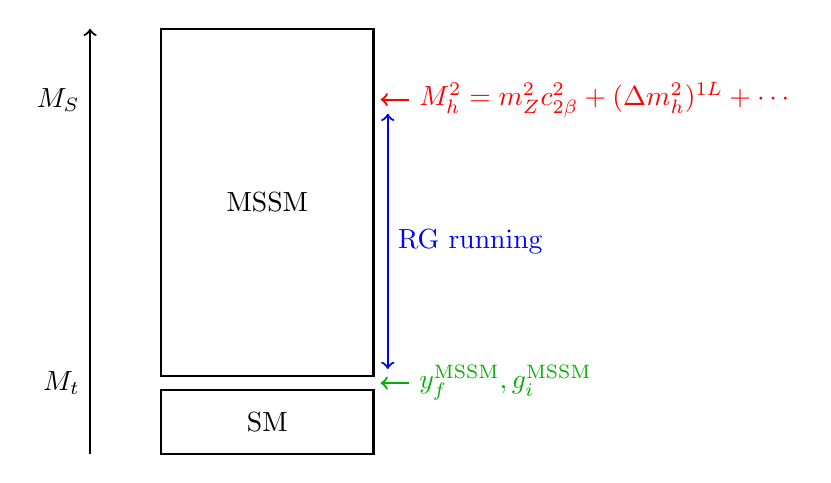
\begin{tikzpicture}[scale=0.9]
      \draw[->, thick] (0,0) -- (0,1) node[left]{$M_t$} -- (0,5) node[left]{$\MS$} -- (0,6);
      \draw[thick] (1,0)   rectangle node{SM}    (4,0.9);
      \draw[thick] (1,1.1) rectangle node{MSSM}  (4,6);
      \draw[<-, thick, red] (4.1,5) -- (4.5,5) node[right]{$M_h^2 = m_Z^2 c_{2\beta}^2 + (\Delta m_h^2)^{1L} + \cdots$};
      \draw[<-, thick, darkgreen] (4.1,1) -- (4.5,1) node[right]{$y_f^\MSSM, g_i^\MSSM$};
      \draw[<->, thick, blue] (4.2,1.2) -- node[right]{RG running} (4.2,4.8);
    \end{tikzpicture}
  \end{center}
\end{frame}

\begin{frame}{Fixed loop order calculation}
  Dominant contribution to $M_h$ at the 1-loop level:
  \begin{align*}
    (\Delta m_h^2)^{1L} &= -\Sigma_h^{1L}(p^2) + \frac{t_h^{1L}}{v} \\
    &= \fmfvcenter{htop} + \fmfvcenter{hstop} + \fmfvcenter{hstopA} \\
    &\phantom{={}} + \fmfvcenter{htoptad} + \fmfvcenter{hstoptad} \\
    &\approx \frac{12 m_t^2 y_t^2}{(4\pi)^2} \left(
      \ln\frac{\MS^2}{m_t^2}
      + \frac{X_t^2}{\MS^2}
      - \frac{X_t^4}{12 \MS^4}
    \right) + O(p^2)
  \end{align*}
\end{frame}

\begin{frame}{Higgs mass at 1-loop level}
  \begin{align*}
    (\Delta m_h^2)^{1L} &\approx
    \frac{12 m_t^2 y_t^2}{(4\pi)^2} \left(
      \ln\frac{\MS^2}{m_t^2}
      + \frac{X_t^2}{\MS^2}
      - \frac{X_t^4}{12 \MS^4}
    \right) + O(p^2)
  \end{align*}
  $X_t = A_t - \mu/t_\beta$ = stop mixing parameter,
  $\MS = (m_Q)_{33} = (m_U)_{33}$
  % 24 mt^4 / (16 Pi^2 v^2) (Log[MS^2/mt^2] + Xt^2/MS^2 - Xt^4/(12 MS^4))
  \\[1em]
  \emph{Observations:}
  \begin{itemize}
  \item logarithmically enhanced by $\MS / m_t$
  \item maximal for $X_t \approx \sqrt{6} \MS$
  \item high sensitivity on $m_t$, due to prefactor $m_t^2 y_t^2 = 2 m_t^4/v^2$
  \item ambiguity of definition of $m_t$: pole mass or \DRbar\ mass? \\
    $M_t \approx 173.3\eh{GeV}$, $m_t^{\DRbar} \approx 165\eh{GeV}$ \\
    $\Rightarrow$ huge theoretical uncertainty!\\
    $\Rightarrow$ 2-loop calculation needed to resolve this ambiguity
  \item $M_h \approx 125\eh{GeV}$ requires $\MS \gtrsim 5\eh{TeV}$
  \end{itemize}
\end{frame}

\begin{frame}{Higgs mass at 2-loop level}
  Known contributions: $O(\as (\at + \ab) + (\at+\ab)^2 + \atau^2)$
  for $p^2 = 0$ \mycite{hep-ph/0105096, hep-ph/0112177}
  \\[1em]
  \includegraphics[width=0.6\textwidth]{images/atas}\\[1em]
  \includegraphics[width=\textwidth]{images/atat}
\end{frame}

\begin{frame}{Higgs mass at 2-loop level}
  \begin{align*}
    (\Delta m_h^2)^{2L} &\approx
    \frac{m_t^2 y_t^4}{(4\pi)^4} \left(
      c_1 \ln^2\frac{\MS^2}{m_t^2}
      + c_2 \ln\frac{\MS^2}{m_t^2}
      + c_3
    \right) \\
    & +
    \frac{m_t^2 y_t^2 g_3^2}{(4\pi)^4} \left(
      c_4 \ln^2\frac{\MS^2}{m_t^2}
      + c_5 \ln\frac{\MS^2}{m_t^2}
      + c_6
    \right)
  \end{align*}
  \emph{Observations:}
  \begin{itemize}
  \item logarithmically enhanced by $\MS / m_t$
  \item still high sensitivity on $m_t$
  \item ambiguity of definition of $m_t$ is resolved \ok
  \item ambiguity of definition of $\as$: $\as^\SM(M_Z)$, $\as^\MSSM(\MS)$, \ldots ? \\
    $\Rightarrow$ 3-loop calculation needed to resolve this ambiguity
  \end{itemize}
\end{frame}

\begin{frame}{Higgs mass at 3-loop level}
  Known contributions: $O(\at\as^2)$ for $p^2 = 0$ \mycite{1005.5709}
  \begin{center}
    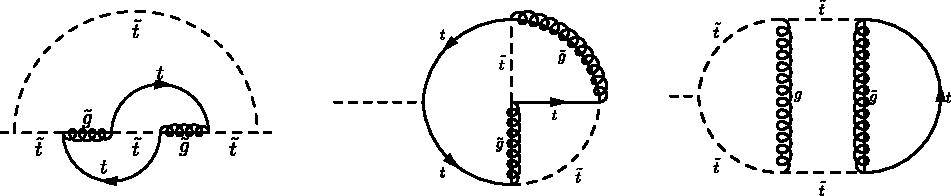
\includegraphics[width=0.9\textwidth]{images/h3l-atasas}
  \end{center}
  \begin{align*}
    (\Delta m_h^2)^{3L} &\approx
    \frac{m_t^2 y_t^2 g_3^4}{(4\pi)^6} \left(
      c_7 \ln^3\frac{\MS^2}{m_t^2}
      + c_8 \ln^2\frac{\MS^2}{m_t^2}
      + c_9 \ln\frac{\MS^2}{m_t^2}
      + c_{10}
    \right)
  \end{align*}
  \emph{Observations:}
  \begin{itemize}
  \item logarithmically enhanced by $\MS / m_t$
  \item still high sensitivity on $m_t$
  \item ambiguity of definition of $m_t$ is resolved \ok
  \item ambiguity of definition of $\as$ is resolved \ok
  \end{itemize}
\end{frame}

\begin{frame}{Summary of fixed loop order calculation}
  Typical order of magnitude of loop contributions (depends on
  parameter scenario):
  \begin{align*}
    M_h &= m_h + \Delta m_h^{1L} + \Delta m_h^{2L} + \Delta m_h^{3L} + \cdots \\
    &\approx [91 + O(20\ldots 30) + O(2\ldots 4) + O(1\ldots 2)] \eh{GeV}
  \end{align*}
  \emph{Advantages:}
  \begin{itemize}
  \item includes logarithmic and non-logarithmic contributions
    % and suppressed terms of
    % $O(v^2/\MS^2)$ at fixed loop order
  \item precise prediction if $\MS \sim m_t$
  \end{itemize}
  \emph{Problem:}
  \begin{itemize}
  \item large logarithmic corrections, if $\MS \gg m_t$ \\
    $\Rightarrow$ slow convergence of perturbation series \\
    $\Rightarrow$ large theoretical uncertainty, ($1$--$2\eh{GeV}$, or
    more)
    % \\
    % recall: $M_h^{\text{exp}} = (125.09 \pm 0.24)\eh{GeV}$
  \end{itemize}
  % \emph{Note:} 3-loop MSSM corrections available in \Himalaya \mycite{1708.05720}
\end{frame}

\begin{frame}{Uncertainty estimate of the fixed-order \DRbarp\ calculation}
  \begin{center}
    \includegraphics[width=0.49\textwidth]{{{plots/SOFTSUSY/SS_TB-20_Xt--sqrt6}}}\hfill
    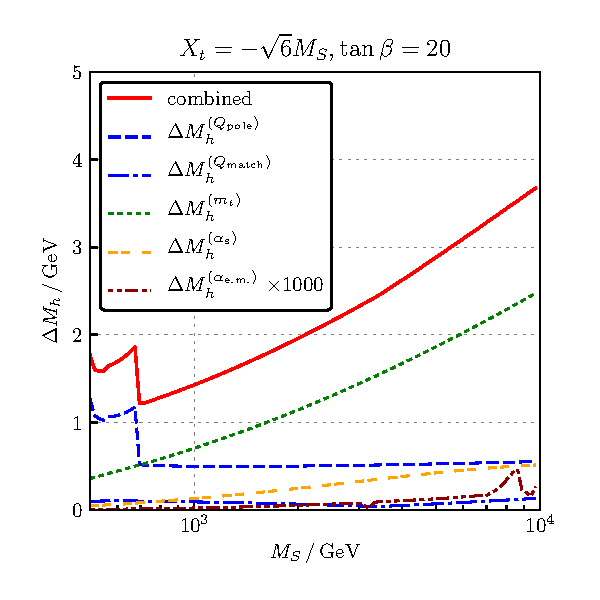
\includegraphics[width=0.49\textwidth]{{{plots/SOFTSUSY/SS_TB-20_Xt--sqrt6_individual}}}
  \end{center}
  \mycite{1804.09410}
\end{frame}

%%% EFT %%%%%%%%%%%%%%%%%%%%%%%%%%%%%%%%%%%%%%%%%%%%%%%

% colored SUSY particles are probably heavy -> this scenario is
% possibly most realistic

% 2. EFT approach: since colored SUSY particles are heavy -> construct
% different EFTs: SM, SM+split, 2HDM, 2HDM+split
%
% a) simplest option: SM-like:
% - pure EFT calculation is possible -> compare to FO!
% - hybrid approach is possible (Flexibleefthiggs or FH-approach)
%   (can be fully automatized due to its simplicity)
%
% b) advanced options: 2HDM-like
% -> show some plots with uncertainty est. from Bagnaschi/Weiglein/Voigt

% Conclusion: In the MSSM EFT calculation is most precise above ~ 1TeV
% Beyond MSSM: not so clear
% Flexibleefthiggs:  very precise and easy to automate
% UOLEA: only 1-loop, but incl. h.o. operators, easy to automate

%%%%%%%%%%%%%%%%%%%%%%%%%%%%%%%%%%%%%%%%

\subsection{Effective field theory calculation}

\begin{frame}{Contents}
  \tableofcontents[currentsection,currentsubsection]
\end{frame}

\begin{frame}{Higgs mass calculation in an EFT}
  \emph{Idea:} Decouple SUSY particles at $\MS$ (expand in $v^2/\MS^2$) \\
  $\Rightarrow$ $\lambda(\MS)$ is fixed by the MSSM \\
  % $\Rightarrow$ effectively: separation of scales $\MS$ and $M_t$.
  \begin{center}
    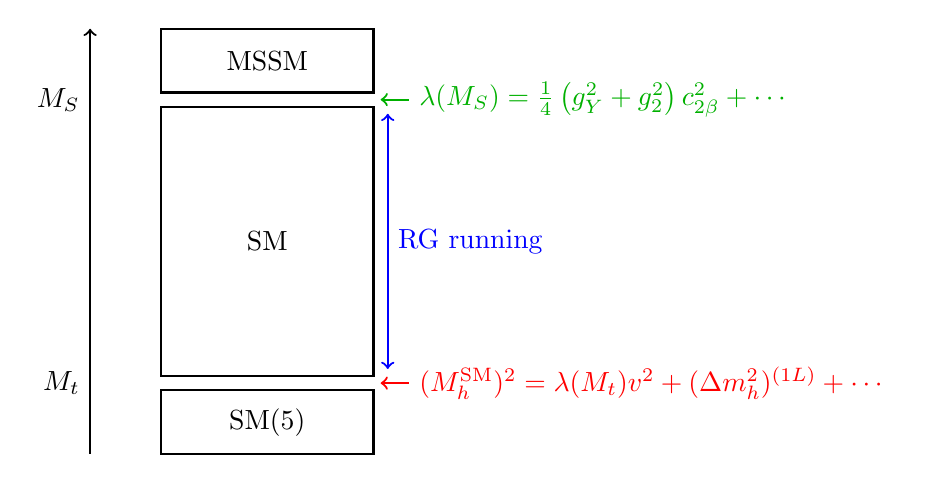
\begin{tikzpicture}[scale=0.9]
      \draw[->, thick] (0,0) -- (0,1) node[left]{$M_t$} -- (0,5) node[left]{$\MS$} -- (0,6);
      \draw[thick] (1,0)   rectangle node{SM(5)} (4,0.9);
      \draw[thick] (1,1.1) rectangle node{SM}    (4,4.9);
      \draw[thick] (1,5.1) rectangle node{MSSM}  (4,6);
      \draw[<-, thick, darkgreen] (4.1,5) -- (4.5,5) node[right]{$\lambda(\MS) = \frac{1}{4}\left(g_Y^{2} + g_2^2\right) c^2_{2\beta} + \cdots$};
      \draw[<-, thick, red] (4.1,1) -- (4.5,1) node[right]{$(M_h^\SM)^2 = \lambda(M_t) v^2 + (\Delta m_h^2)^{(1L)} + \cdots$};
      \draw[<->, thick, blue] (4.2,1.2) -- node[right]{RG running} (4.2,4.8);
    \end{tikzpicture}
  \end{center}
\end{frame}

% \begin{frame}{EFT avoids large logarithmic corrections}
%   \begin{enumerate}
%   \item Calculate $\lambda$ from the condition ($p^2 = v^2 = 0$):
%     \begin{align*}
%       \partial_{p^2}^{(k)}\Gamma_{h,\ldots,h}^{\MSSM,(n)}
%       = \partial_{p^2}^{(k)}\Gamma_{h,\ldots,h}^{\SM,(n)}
%     \end{align*}
%     $\Rightarrow$
%     \begin{align*}
%       \lambda(Q) &= \frac{1}{4}\left[g_Y^{2} + g_2^2\right] c^2_{2\beta}
%                    + \Delta \lambda^{1L} + \Delta \lambda^{2L} + \cdots \\
%                  &= \frac{1}{4}\left[g_Y^{2} + g_2^2\right] c^2_{2\beta}
%       + \frac{12 m_t^2 y_t^2}{(4\pi)^2 v^2} \left[
%         \ln\frac{\MS^2}{Q^2} + \frac{X_t^2}{\MS^2} - \frac{X_t^4}{12 \MS^4}
%       \right]
%       + \cdots
%     \end{align*}
%     $\Rightarrow$ \textcolor{darkgreen}{no large logs for $Q\approx\MS$}
%   \item RG running of $\lambda$ from $Q = \MS$ $\rightarrow M_t$.\\
%     $\Rightarrow$ \textcolor{darkgreen}{logs are resummed to all orders}
%   \item Calculate $M_h$ in the SM at $Q = M_t$:
%     \begin{align*}
%       (M_h^\SM)^2 &= \lambda(Q) v^2 + \frac{12 m_t^2 y_t^2}{(4\pi)^2 v^2} \ln\frac{Q^2}{m_t^2} + \cdots
%     \end{align*}
%     $\Rightarrow$ \textcolor{darkgreen}{no large logs for $Q\approx M_t$}
%   \end{enumerate}
% \end{frame}

\begin{frame}{Summary of EFT approach}
  Typical order of magnitude of loop contributions (depends on
  parameter scenario, here $X_t = 0$, $\MS = 20\eh{TeV}$):
  \begin{align*}
    M_h &= m_h + \Delta m_h^{1L} + \Delta m_h^{2L} + \Delta m_h^{3L} + \cdots \\
    % &= \sqrt{\lambda(M_t)} v + \Delta m_h^{1L} + \Delta m_h^{2L} + \cdots \\
    &\approx [O(124) + O(0.5\ldots 1) + O(0.1\ldots 0.2) + O(0.02\ldots 0.04)] \eh{GeV}
    % &= \sqrt{\lambda(\MS)} v + \text{logs} + \Delta m_h^{1L} + \Delta m_h^{2L} + \cdots \\
    % &\approx [O(84) + O(40) + O(0.5\ldots 1) + O(0.1\ldots 0.2)] \eh{GeV}
  \end{align*}
  \emph{Advantages:}
  \begin{itemize}
  \item large logarithmic fixed order loop corrections are avoided
  \item large logarithms $\propto\ln(M_S/M_t)$ are resummed to all orders
  \end{itemize}
  \emph{Disadvantage:} terms of $O(v^2/M_S^2)$ are neglected \\
  $\Rightarrow$ imprecise when $v \sim \MS$ \\
  $\Rightarrow$ large theoretical uncertainty when $v \sim \MS$
\end{frame}

\begin{frame}{Comparison of fixed-order and EFT calculation}
  \begin{center}
    \includegraphics[width=0.49\textwidth]{plots/SOFTSUSY/Mh_MS_TB-20_Xt--sqrt6}\hfill
    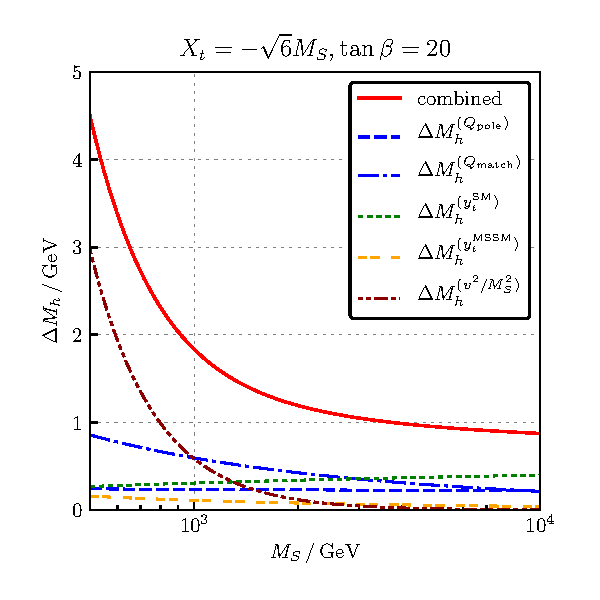
\includegraphics[width=0.49\textwidth]{plots/SOFTSUSY/HSSUSY_TB-20_Xt--sqrt6_individual}
  \end{center}
  \begin{center}
    $\DMh \overset{!}{=} \DMhHSSUSY$\\[0.5em]
    $\Rightarrow$ $\MS^{\text{equal}} = 1.0$--$1.3\TeV$ for
    small/large $\tan\beta$ and/or $X_t$
  \end{center}
  \mycite{1804.09410}
\end{frame}

\begin{frame}{Summary of fixed-order and EFT approaches}
  \begin{center}
    \begin{tabular}{lcc}
      \toprule
                  & low $\MS$ & high $\MS$ \\
                  & $\MS \lesssim 1\eh{TeV}$ & $\MS \gtrsim 1\eh{TeV}$ \\
      \midrule
      fixed-order & \ok       & \notok     \\
      EFT         & \notok    & \ok        \\
      ? mixed     & \ok       & \ok        \\
      \bottomrule
    \end{tabular}
  \end{center}
  \vspace{2em}
  Q: Can the fixed-order and EFT approaches be combined? \\[1em]
  A: Yes!  \mycite{1312.4937, 1609.00371, 1710.03760}
\end{frame}

%%%%%%%%%%%%%%%%%%%%%%%%%%%%%%%%%%%%%%%%

\subsection{Hybrid fixed-order/EFT calculation}

\begin{frame}{Contents}
  \tableofcontents[currentsection,currentsubsection]  
\end{frame}

\begin{frame}{Hybrid fixed-order/EFT calculation}
  \emph{Goal:} resum large logarithms \emph{and} include suppressed
  $O(v^2/\MS^2)$ terms
  \\[2em]
  \emph{Idea I:} (``FeynHiggs approach'' \mycite{1312.4937, 1706.00346, 1805.00867})\\
  Replace logs from fixed-order calculation by resummed logs:
  \begin{align*}
    M_h^2 = (M_h^2)_{\text{fixed-order}} - (M_h^2)_{\text{logs}} + (M_h^2)_{\text{resummed logs}}
  \end{align*}
  \emph{Pro:}
  \begin{itemize}
  \item[\ok] approach applicable to any BSM model
  \item[\ok] any EFT can be used
  \end{itemize}
  \emph{Contra:}
  \begin{itemize}
  \item[\notok] requires knowledge of fixed-order and EFT expressions
  \item[\notok] care must be taken to avoid double counting
  \end{itemize}
\end{frame}

\begin{frame}{Hybrid fixed-order/EFT calculation}
  % \emph{Goal:} resum large logarithms \emph{and} include suppressed
  % $O(v^2/\MS^2)$ terms
  % \\[2em]
  \emph{Idea II:} (``FlexibleEFTHiggs'' \mycite{1609.00371,
    1710.03760})\\
  Incorporate $O(v^2/\MS^2)$ terms into $\lambda$ by using the
  matching condition
  \begin{align*}
    (M_h^2)_{\SM} &\overset{!}{=} (M_h^2)_{\BSM} \qquad \text{at } Q = \MS \\
    \lambda(\MS) v^2 + (\Delta m_h^2)_{\SM} &= (M_h^2)_{\BSM}
  \end{align*}
  $\Rightarrow$
  \begin{align*}
    \lambda(\MS) = \frac{1}{v^2}\left[(M_h^2)_{\BSM} - (\Delta m_h^2)_{\SM}\right]
  \end{align*}
  Continue as in in the EFT calculation \ldots
  % \emph{Pro:}
  % \begin{itemize}
  % \item[\ok] approach applicable to any BSM model
  %   % easy to apply to any SM extensison
  % \item[\ok] easy to automate
  %   (only fixed-order expressions required)
  % \end{itemize}
  % \emph{Contra:}
  % \begin{itemize}
  % \item[\notok] difficult to extend to other EFTs beyond the SM (2HDM,
  %   \ldots)
  % \item[\meh] tricky to reach 2-loop accuracy\\
  %   (requires careful treatment of parameter matching)
  % \end{itemize}
\end{frame}

\begin{frame}{FlexibleEFTHiggs approach}
  Continue as in the EFT calculation:
  \begin{center}
    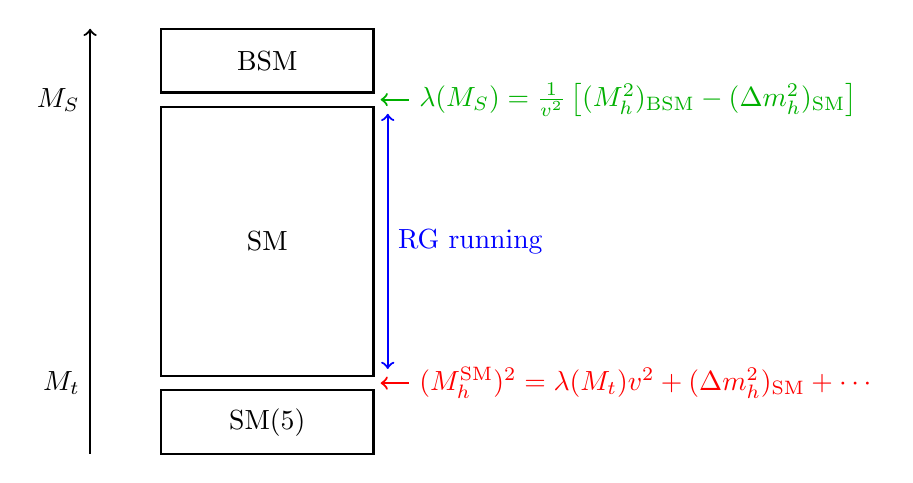
\begin{tikzpicture}[scale=0.9]
      \draw[->, thick] (0,0) -- (0,1) node[left]{$M_t$} -- (0,5) node[left]{$\MS$} -- (0,6);
      \draw[thick] (1,0)   rectangle node{SM(5)} (4,0.9);
      \draw[thick] (1,1.1) rectangle node{SM}    (4,4.9);
      \draw[thick] (1,5.1) rectangle node{BSM}  (4,6);
      \draw[<-, thick, darkgreen] (4.1,5) -- (4.5,5) node[right]{$\lambda(\MS) = \frac{1}{v^2}\left[(M_h^2)_{\BSM} - (\Delta m_h^2)_{\SM}\right]$};
      \draw[<-, thick, red] (4.1,1) -- (4.5,1) node[right]{$(M_h^\SM)^2 = \lambda(M_t) v^2 + (\Delta m_h^2)_{\SM} + \cdots$};
      \draw[<->, thick, blue] (4.2,1.2) -- node[right]{RG running} (4.2,4.8);
    \end{tikzpicture}
  \end{center}
\end{frame}

\begin{frame}{FlexibleEFTHiggs approach}
  Matching condition:
  \begin{align*}
    (M_h^2)_{\SM} &\overset{!}{=} (M_h^2)_{\BSM}
  \end{align*}
  \emph{Pro:}
  \begin{itemize}
  \item[\ok] approach applicable to any BSM model
    % easy to apply to any SM extensison
  \item[\ok] very simple $\rightarrow$ easy to automate
  \item[\ok] only BSM fixed-order expressions required
  \end{itemize}
  \emph{Contra:}
  \begin{itemize}
  \item[\notok] difficult to extend to other EFTs beyond the SM (2HDM,
    \ldots)
  \item[\meh] tricky to reach 2-loop accuracy\\
    (requires careful treatment of parameter matching)
  \end{itemize}
\end{frame}

\begin{frame}{Comparison of the three approaches in the MSSM}
  % Currently NLO + NLL is available \mycite{1609.00371, 1710.03760}.\\
  % Extension to NNLO + NNLL is work in progress:
  \begin{center}
    \includegraphics[width=0.49\textwidth]{{{plots/FlexibleEFTHiggs-2L/Mh_MS_TB-20_Xt-0}}}
    \hfill
    \includegraphics[width=0.49\textwidth]{{{plots/FlexibleEFTHiggs-2L/Mh_MS_TB-20_Xt--sqrt6}}}
  \end{center}
  Preliminary work by Thomas Kwasnitza, Dominik Stöckinger, AV
\end{frame}

%%%%%%%%%%%%%%%%%%%%%%%%%%%%%%%%%%%%%%%%

\section{Where is SUSY?}

\begin{frame}{Contents}
  \tableofcontents[currentsection]  
\end{frame}

\begin{frame}{Where is SUSY?}
  Difficult question!\\[1em]
  $\rightarrow$ Need to make precise predictions for all parameter scenarios\\[1em]
  $\rightarrow$ Need to consider all different kinds of EFTs!
\end{frame}

\begin{frame}{Scenarios with 1 light Higgs doublet}
  \begin{center}
    \begin{tikzpicture}[scale=0.8, every node/.style={transform shape}]
      \draw[->, thick] (0,0) -- (0,1) node[left]{$M_t$} -- (0,4) node[left]{$\MS$} -- (0,6);
      \node at (2.5,7) {\emph{I high-scale SUSY}};
      \draw[thick] (1,0)   rectangle node{SM}    (4,0.9);
      \draw[thick] (1,1.1) rectangle node{SM}   (4,4.9);
      \draw[thick] (1,5.1) rectangle node{MSSM}  (4,6);
      % 
      \node at (6.5,7) {\emph{II split-SUSY}};
      \draw[thick] (5,0)   rectangle node{SM}    (8,1.9);
      \draw[thick] (5,2.1) rectangle node{SM + $\chi_i$ + $\tilde{g}$} (8,4.9);
      \draw[thick] (5,5.1) rectangle node{MSSM}  (8,6);
    \end{tikzpicture}
  \end{center}
\end{frame}

\begin{frame}{Scenarios with 2 light/intermediate Higgs doublets}
  \begin{center}
    \begin{tikzpicture}[scale=0.8, every node/.style={transform shape}]
      \draw[->, thick] (0,0) -- (0,1) node[left]{$M_t$} -- (0,4) node[left]{$\MS$} -- (0,6);
      \node[align=center] at (2.5,7) {\emph{III 2HDM}\\ (light $h_i$, $A$, $H^{\pm}$)};
      \draw[thick] (1,0)   rectangle node{SM} (4,0.9);
      \draw[thick] (1,1.1) rectangle node{2HDM} (4,4.9);
      \draw[thick] (1,5.1) rectangle node{MSSM} (4,6);
      % 
      \node[align=center] at (6.5,7) {\emph{IV 2HDM+split}\\ (light $h_i$, $A$, $H^{\pm}$,\\ intermediate $\chi_i$, $\tilde{g}$)};
      \draw[thick] (5,0)   rectangle node{SM} (8,0.9);
      \draw[thick] (5,1.1) rectangle node{2HDM} (8,2.9);
      \draw[thick] (5,3.1) rectangle node[align=center]{2HDM\\ + $\chi_i$ + $\tilde{g}$} (8,4.9);
      \draw[thick] (5,5.1) rectangle node{MSSM} (8,6);
      % 
      \node[align=center] at (10.5,7) {\emph{V 2HDM+split}\\ (light $\chi_i$, $\tilde{g}$, inter-\\ mediate $h_2$, $A$, $H^{\pm}$)};
      \draw[thick] (9,0)   rectangle node{SM} (12,0.9);
      \draw[thick] (9,1.1) rectangle node{SM + $\chi_i$ + $\tilde{g}$} (12,2.9);
      \draw[thick] (9,3.1) rectangle node[align=center]{2HDM\\ + $\chi_i$ + $\tilde{g}$} (12,4.9);
      \draw[thick] (9,5.1) rectangle node{MSSM} (12,6);
    \end{tikzpicture}
  \end{center}
\end{frame}

\begin{frame}{Where is SUSY?}
  \begin{center}
    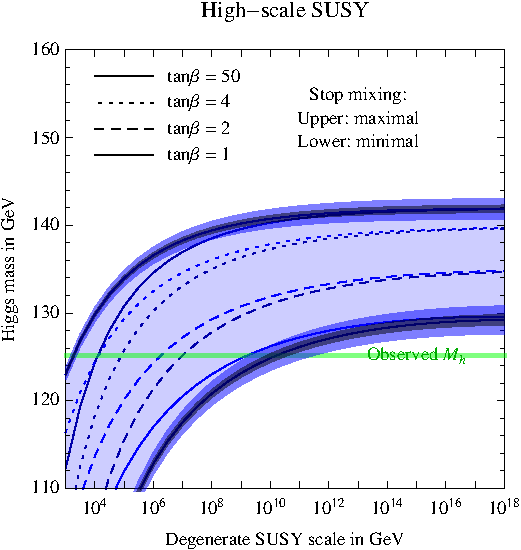
\includegraphics[width=0.49\textwidth]{plots/Where_is_SUSY/HeavySUSY}\hfill
    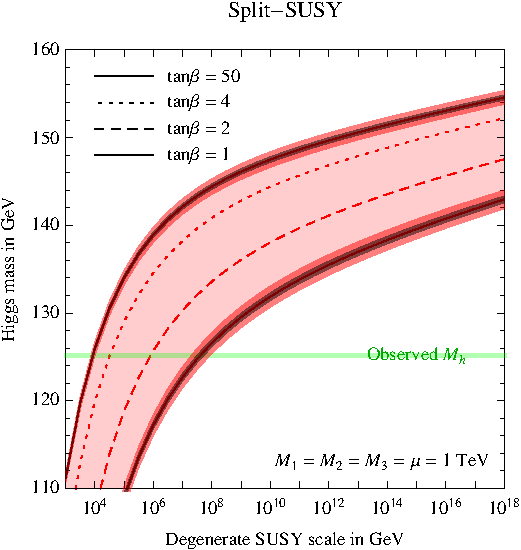
\includegraphics[width=0.49\textwidth]{plots/Where_is_SUSY/SplitSUSY}
  \end{center}
  \mycite{1407.4081}
\end{frame}

%%%%%%%%%%%%%%%%%%%%%%%%%%%%%%%%%%%%%%%%

\section{Summary}

\begin{frame}{Summary}
  \emph{Supersymmetry} is still attractive and viable, but
  $\MS \gtrsim 1\TeV$ required in the MSSM to get $M_h = 125.09\GeV$.
  \\[1em]
  \emph{Higgs mass prediction} can be used to constrain SUSY parameter
  space.
  \\[1em]
  \emph{When to use fixed-order/EFT calculation?}
  \begin{itemize}
  \item $\MS \lesssim 1\TeV$ $\Rightarrow$ use fixed-order
  \item $\MS \gtrsim  1\TeV$ $\Rightarrow$ use EFT
  \end{itemize}
  %
  \vspace{1em}
  \emph{Recent advances in EFT calculations:}
  \begin{center}
    \resizebox{0.7\textwidth}{!}{
    \begin{tabular}{lll}
      \toprule
      Model $\rightarrow$ EFT & Accuracy & Program \\
      \midrule
      MSSM $\rightarrow$ SM           & N$^3$LO + N$^3$LL & FS \\
      MSSM $\rightarrow$ split-SUSY   & N$^2$LO + NLL & FS, FH \\
      MSSM $\rightarrow$ 2HDM(+split) & N$^2$LO + NLL & FS, FH \\
      any BSM $\rightarrow$ SM        & NLO + NLL & FS, SP$^*$ \\
      any BSM $\rightarrow$ any EFT   & NLO + NLL & SP \\
      \bottomrule
    \end{tabular}}
  \end{center}
\end{frame}

\begin{frame}{Prospects}
  \begin{center}
    \LARGE large zoo of models $\Rightarrow$ automation necessary!
  \end{center}
  \begin{center}
    \includegraphics[width=0.9\textwidth]{images/FS.png}
  \end{center}
\end{frame}

%%%%%%%%%%%%%%%%%%%%%%%%%%%%%%%%%%%%%%%%
% backup slides
%%%%%%%%%%%%%%%%%%%%%%%%%%%%%%%%%%%%%%%%

\begin{frame}[noframenumbering]
  \begin{center}
    \Huge Backup
  \end{center}
\end{frame}

%%%%%%%%%%%%%%%%%%%%%%%%%%%%%%%%%%%%%%%%

\begin{frame}[noframenumbering]{Higgs masses in the SM}
  Higgs potential
  \begin{align*}
    V_{\text{Higgs}} = -\mu^2 |\Phi|^2 + \frac{\lambda}{2}|\Phi|^4
    = -\frac{\mu^2}{2} (v+h)^2 + \frac{\lambda}{8} (v+h)^4 + \cdots
  \end{align*}
  where
  \begin{align*}
    \Phi =
    \begin{pmatrix}
      0 \\ \frac{1}{\sqrt{2}} (v + h)
    \end{pmatrix}
  \end{align*}
  After eliminating $\mu^2$:
  \begin{align*}
    V_{\text{Higgs}} = \lambda v^2 \frac{h^2}{2} + \cdots
    \qquad\Rightarrow\qquad
    m_h^2 = \lambda v^2  \qquad \text{(tree-level)}
  \end{align*}
  \emph{Until 2012:} $M_h =\ ?$ $\Leftrightarrow$ $\lambda =\ ?$\\
  \emph{Since 2012:} $M_h \approx 125\eh{GeV}$ $\Rightarrow$ $\lambda \approx 0.26$
\end{frame}

%%%%%%%%%%%%%%%%%%%%%%%%%%%%%%%%%%%%%%%%

\begin{frame}[noframenumbering]{Higgs masses in the (real) MSSM}
  Higgs potential:
  \begin{align*}
    V_{\text{Higgs}} = \frac{1}{8}(g_Y^2 + g_2^2)(|h_1|^2 - |h_2|^2)^2 + \frac{g_2^2}{2}|h_1^\dagger h_2|^2 + \cdots
  \end{align*}
  where
  \begin{align*}
    % h, H, A, H^\pm
    h_1 =
    \begin{pmatrix}
      \frac{1}{\sqrt{2}} (v_1 + h_1^0) \\ 0
    \end{pmatrix}, \qquad
    h_2 =
    \begin{pmatrix}
      0 \\ \frac{1}{\sqrt{2}} (v_2 + h_2^0)
    \end{pmatrix}
  \end{align*}
  After EWSB (if $m_A \gg m_Z$):
  \begin{align*}
    V_{\text{Higgs}} \approx \frac{1}{4}(g_Y^2+g_2^2) v^2 c_{2\beta}^2 \frac{h^2}{2} + \cdots
    = m_Z^2 c_{2\beta}^2 \frac{h^2}{2} + \cdots
    % m_h^2 = \frac{1}{2} \left[
    %   m_Z^2 + m_A^2 - \sqrt{(m_Z^2 + m_A^2)^2 - 4 m_Z^2 m_A^2 \cos^2{2\beta}}
    % \right]
  \end{align*}
  $\Rightarrow$ \emph{prediction}:
  \begin{align*}
    m_h^2 = m_Z^2 \cos^2{2\beta}
    % = \frac{1}{4} (g_Y^2 + g_2^2) v^2 \cos^2{2\beta}
    \leq m_Z^2
    \approx (91.2 \eh{GeV})^2  \qquad \text{(tree-level)}
  \end{align*}
\end{frame}

%%%%%%%%%%%%%%%%%%%%%%%%%%%%%%%%%%%%%%%%


\begin{frame}[noframenumbering]{Where is SUSY?}
  \begin{center}
    \emph{I high-scale SUSY}\\[0.5em]
    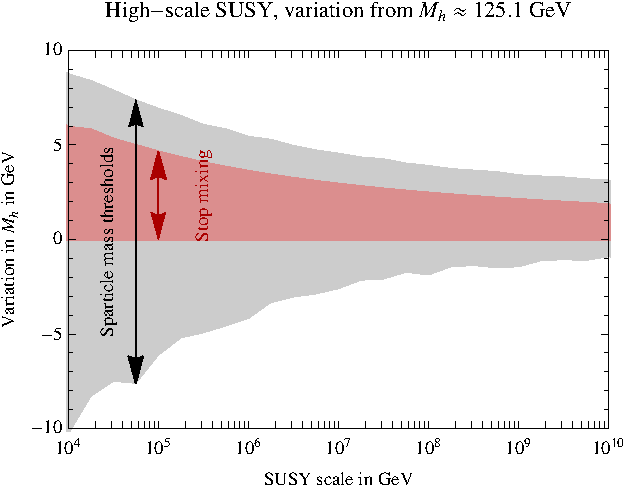
\includegraphics[width=0.7\textwidth]{{{plots/Where_is_SUSY/Mhband}}}
  \end{center}
  \mycite{1407.4081}
\end{frame}

\begin{frame}[noframenumbering]{Where is SUSY?}
  \begin{center}
    \emph{IV THDM+split}\\[0.5em]
    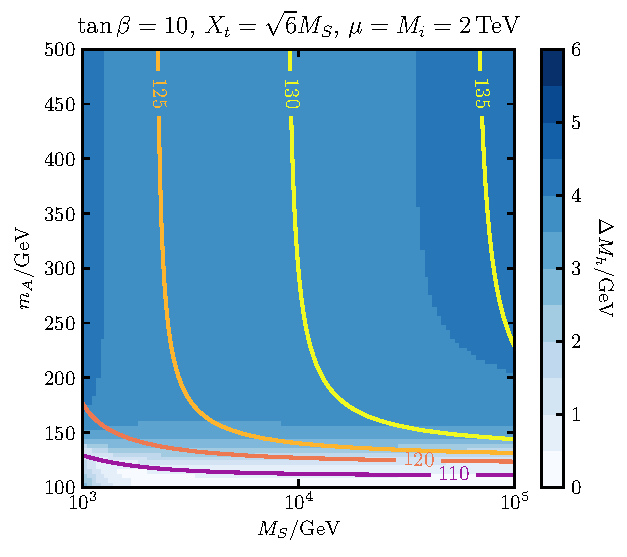
\includegraphics[width=0.6\textwidth]{{{plots/THDM/SplitTHDMTHDMTower_MS_MA_Xt-2.44949_TB-10_Mu-M12-M3-2000}}}
  \end{center}
\end{frame}

%%%%%%%%%%%%%%%%%%%%%%%%%%%%%%%%%%%%%%%%

\begin{frame}[noframenumbering]{Current status of (N)MSSM spectrum generators}
  \begin{center}
    \emph{MSSM}\\[0.4em]
    \begin{tabular}{llll}
      \toprule
      Spectrum generator & fixed order & EFT & hybrid \\
      \midrule
      \FH                & 2L & 2L & NNLO + NNLL \\
      \FS                & \textcolor{darkgreen}{3L} & \textcolor{darkgreen}{3L} & \textcolor{darkgreen}{NNLO + NNLL}$^\dagger$ \\
      \SOFTSUSY          & \textcolor{darkgreen}{3L} & -- & -- \\
      \SARAH/\SPheno     & 2L & -- & NNLO + LL \\
      \bottomrule
    \end{tabular}
  \end{center}
  %
  \begin{center}
    \emph{NMSSM}\\[0.4em]
    \begin{tabular}{llll}
      \toprule
      Spectrum generator & fixed order & EFT & hybrid \\
      \midrule
      \FH                & -- & -- & -- \\
      \FS                & 2L$^*$ & -- & \textcolor{darkgreen}{NNLO + NNLL}$^\dagger$ \\
      \SOFTSUSY          & 2L$^*$ & -- & -- \\
      \SARAH/\SPheno     & 2L & 1L & NNLO + LL \\
      \bottomrule
    \end{tabular}
  \end{center}
  $^\dagger$ in preparation\\
  $^*$ $O(\at^2)$ corrections in the MSSM limit, no $O(\at\lambda^2)$ corrections
\end{frame}

%%%%%%%%%%%%%%%%%%%%%%%%%%%%%%%%%%%%%%%%

\begin{frame}[noframenumbering]{Uncertainty estimate of the fixed-order \DRbarp\ calculation}
  Calculation of $m_t$ in two different ways as proposed in
  \bigcite{1609.00371}:
  \begin{align*}
    m_t^{[1]} &=
                M_t + \widetilde{\Sigma}_t^{(1L),S} +
                M_t \left[
                \widetilde{\Sigma}_t^{(1L),L} +
                \widetilde{\Sigma}_t^{(1L),R}
                \right] \\
              &\phantom{={}} + M_t
                \left[\widetilde{\Sigma}_t^{(1L),\SQCD}
                + \widetilde{\Sigma}_t^{(2L),\SQCD}
                + \left(\widetilde{\Sigma}_t^{(1L),\SQCD}\right)^2
                \right]\\
    m_t^{[2]} &=
                M_t + \widetilde{\Sigma}_t^{(1L),S} +
                m_t \left[
                \widetilde{\Sigma}_t^{(1L),L} +
                \widetilde{\Sigma}_t^{(1L),R}
                \right] \nonumber \\
              &\phantom{={}} +
                m_t
                \left[\widetilde{\Sigma}_t^{(1L),\SQCD} +
                \widetilde{\Sigma}_t^{(2L),\SQCD}
                \right]
  \end{align*}
  Calculation of $\as$ and $\aem$ in two different ways:
  \begin{align*}
    \as^{[1]}  &= \frac{\as^{\SM(5)}}{1 - \Delta^{(1L)}\as - \Delta^{(2L)}\as}\\
    \as^{[2]}  &= \as^{\SM(5)} \left[1 + \Delta^{(1L)}\as + (\Delta^{(1L)}\as)^2 + \Delta^{(2L)}\as\right]
  \end{align*}
\end{frame}

%%%%%%%%%%%%%%%%%%%%%%%%%%%%%%%%%%%%%%%%

\begin{frame}[noframenumbering]{Uncertainty estimate of FlexibleEFTHiggs-1L}
  \begin{align*}
    \DMhQpole &= \max_{\Qpole\in[M_t/2,2M_t]}\left|M_h(\Qpole) - M_h(M_t)\right| & \text{\mycite{1609.00371}} \\
    \DMhQmatch &= \max_{\Qmatch\in[\MS/2,2\MS]}\left|M_h(\Qmatch) - M_h(\MS)\right| & \text{\mycite{1407.4081}} \\
    \DMhHSSUSYytSM &= \left| M_h(y_t^{\SM,(2L)}(M_Z)) - M_h(y_t^{\SM,(3L)}(M_Z)) \right| & \text{\mycite{1504.05200}} \\
    \DMhEFT &= 0 \quad \text{(has no EFT uncertainty!)} & \text{\mycite{1609.00371}}
  \end{align*}
\end{frame}

%%%%%%%%%%%%%%%%%%%%%%%%%%%%%%%%%%%%%%%%

\begin{frame}[noframenumbering]{Uncertainty estimate of fixed-order \DRbarp\ calculation}
  In \bigcite{1804.09410} 5 sources of uncertainty were combined:
  \begin{align*}
    \DMhQpole &= \max_{\Qpole\in[\MS/2,2\MS]}\left|M_h(\Qpole) - M_h(\MS)\right| & \text{\mycite{1609.00371}} \\
    \DMhQmatch &= \max_{\Qmatch\in[M_Z/2,2M_Z]}\left|M_h(\Qmatch) - M_h(M_Z)\right| & \text{\mycite{\underline{1804.09410}}} \\
    \DMhMt &= \left|M_h(m_t^{[1]}) - M_h(m_t^{[2]})\right| & \text{\mycite{1609.00371}} \\
    \DMhAlphaS &= \left| M_h(\as^{[1]}) - M_h(\as^{[2]}) \right| & \text{\mycite{\underline{1804.09410}}} \\
    \DMhAlphaEm &= \left| M_h(\aem^{[1]}) - M_h(\aem^{[2]}) \right| & \text{\mycite{\underline{1804.09410}}}
  \end{align*}
  Combination:
  \begin{align*}
    \DMh &= \DMhQpole + \DMhQmatch + \DMhMt + \DMhAlphaS + \DMhAlphaEm 
  \end{align*}
\end{frame}

%%%%%%%%%%%%%%%%%%%%%%%%%%%%%%%%%%%%%%%%

\begin{frame}[noframenumbering]{Uncertainty estimate of the EFT calculation}
  In \bigcite{1804.09410} 5 sources of uncertainty were combined:
  \begin{align*}
    \DMhQpole &= \max_{\Qpole\in[M_t/2,2M_t]}\left|M_h(\Qpole) - M_h(M_t)\right| & \text{\mycite{1609.00371}} \\
    \DMhQmatch &= \max_{\Qmatch\in[\MS/2,2\MS]}\left|M_h(\Qmatch) - M_h(\MS)\right| & \text{\mycite{1407.4081}} \\
    \DMhHSSUSYytSM &= \left| M_h(y_t^{\SM,(2L)}(M_Z)) - M_h(y_t^{\SM,(3L)}(M_Z)) \right| & \text{\mycite{1504.05200}} \\
    \DMhEFT &= \left| M_h - M_h(v^2/\MS^2) \right| & \text{\mycite{1504.05200}} \\
    \DMhHSSUSYytMSSM &= \left| M_h - M_h(y_t^\MSSM(\MS)) \right| & \text{\mycite{Bagnaschi,AV,Weiglein}}
  \end{align*}
  Combination:
  \begin{align*}
    \DMhHSSUSY &= \DMhQpole + \DMhQmatch + \DMhHSSUSYytSM + \DMhHSSUSYytMSSM \\
    &\quad + \DMhEFT
  \end{align*}
\end{frame}

%%%%%%%%%%%%%%%%%%%%%%%%%%%%%%%%%%%%%%%%

\begin{frame}[noframenumbering]{Effect of the 3-loop $O(\at\as^2)$ corrections to $M_h$}
  \begin{center}
    \includegraphics[width=0.49\textwidth]{plots/SOFTSUSY/Mh_2L_vs_3L_MS_TB-20_Xt--sqrt6}\hfill
    \includegraphics[width=0.49\textwidth]{plots/Mh3L/scan_Mh_MS_TB-20_Xt--sqrt6_uncertainty_Qpole}
  \end{center}
  \mycite{1708.05720}
\end{frame}

%%%%%%%%%%%%%%%%%%%%%%%%%%%%%%%%%%%%%%%%

\begin{frame}[noframenumbering]{Effect of the 3-loop corrections to $\lambda(\MS)$}
  3-loop corrections to $\lambda(\MS)$ allow for an N$^3$LL
  resummation of strong corrections $O(\at^2\as^2)$:
  \begin{center}
    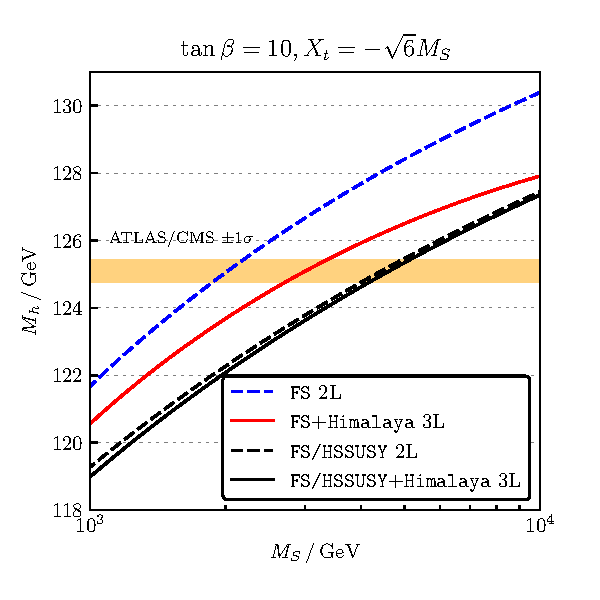
\includegraphics[width=0.49\textwidth]{plots/HSSUSY-3L/scan_Mh_MS_TB-10_Xt--sqrt6}\hfill
    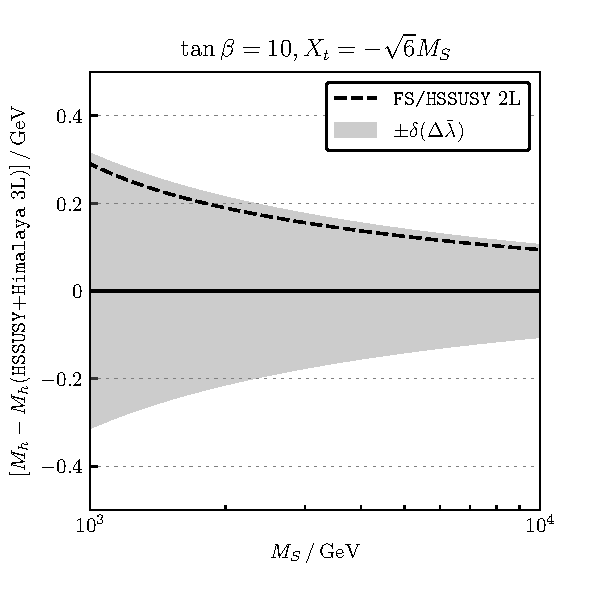
\includegraphics[width=0.49\textwidth]{plots/HSSUSY-3L/scan_Mh_MS_TB-10_Xt--sqrt6_diff}
  \end{center}
  \mycite{1807.03509}
\end{frame}

%%%%%%%%%%%%%%%%%%%%%%%%%%%%%%%%%%%%%%%%

\begin{frame}[noframenumbering]{Fixed-order vs.\ hybrid calculation in the NMSSM}
  \begin{center}
    \includegraphics[width=0.4\textwidth]{{{plots/NMSSMEFTHiggs/DMh_MS_TB-5_Xt-0_lam-0.1_kap-0.1}}}%\hfill
    \includegraphics[width=0.4\textwidth]{{{plots/NMSSMEFTHiggs/DMh_MS_TB-5_Xt-0_lam-0.3_kap-0.3}}}\\
    \includegraphics[width=0.4\textwidth]{{{plots/NMSSMEFTHiggs/DMh_MS_TB-5_Xt--2_lam-0.1_kap-0.1}}}%\hfill
    \includegraphics[width=0.4\textwidth]{{{plots/NMSSMEFTHiggs/DMh_MS_TB-5_Xt--2_lam-0.3_kap-0.3}}}
  \end{center}
\end{frame}

%%%%%%%%%%%%%%%%%%%%%%%%%%%%%%%%%%%%%%%%

\begin{frame}[noframenumbering]{Gauge Coupling Unification}
  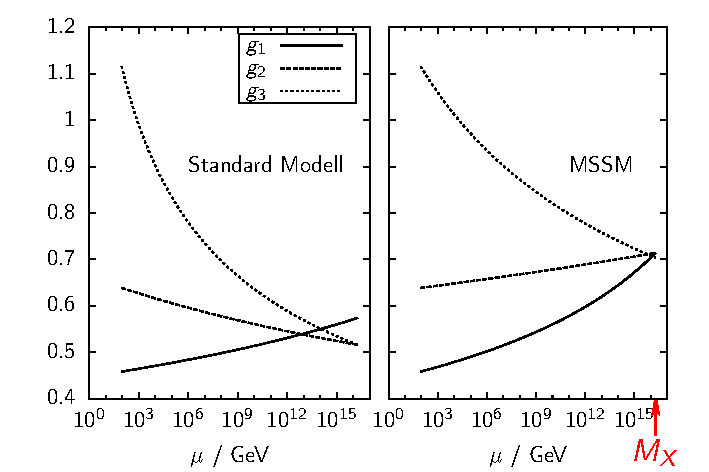
\includegraphics[width=\textwidth]{images/MSSM_gauge_couplings_largeMX}
\end{frame}

\end{document}
